\documentclass[12pt]{article}
\usepackage[margin=1.5cm]{geometry}
\linespread{1.5}
\usepackage{listings}
\usepackage{xcolor}
\usepackage{graphicx}
\usepackage{tikz}
\usepackage{tcolorbox}
\usepackage{hyperref}
\tcbuselibrary{listings, skins}

\definecolor{maincs}{RGB}{0,255,0}
\definecolor{secondarycs}{RGB}{255,179,246}

\newcommand\tab[1][.5in]{\hspace*{#1}}

\lstset{
    language=Python,
        numbers=left,
        numberstyle=\small,
        numbersep=8pt,
        frame=single,
        framexleftmargin=15pt,
        basicstyle=\fontsize{9}{10}\ttfamily,
        otherkeywords={self,import,from},
        keywordstyle=\color{purple}\ttfamily,
        emph={True,False},
        emphstyle=\color{orange},
        stringstyle=\color{red}\ttfamily,
        commentstyle=\color{blue}\ttfamily,
        morecomment=[l][\color{blue}]{\#},
        tabsize=2,
        showstringspaces=false
}

\begin{document}
\begin{titlepage}
\vspace*{\fill}
{
    \centering
    \bfseries
    \emph{\Huge Grandfather's Maze Algorithm Report}
    \vskip 1.5in

    \Large Robbie Merillat \\
    \vskip 2in

    26 April 2017

}
\vspace*{\fill}
\clearpage
\end{titlepage}

\section{Modeling the Problem}~\\
\tab The first step that I took in approaching this problem was to attempt to solve the problem of traversing from Startsburg to Endenville by hand, just as the grandfather had in the past. This was both to determine a path that worked and find the number of edges that it would move along to solve it. Thus I would have some baseline answer that I could compare the result of my algorithm to in order to determine its' correctness. I started from the end point and worked my way backwards, just as a backtrace in an algorithm might, and determined a path that took 49 steps to complete.\\
\tab After finding the number of steps, the next challenge that I tackled was modeling the graph that the Grandfather had used as some form of data structure within a python script. I determined that sorting each maze node as a literal node in the code, may not be the best as it would have to have some sort of value to store whether it was traveled in one direction and in a backwards direction. This would have been trivial to create, however, down the line, the BFS would have to traverse and use some grueling logic to keep track of where it had been and where it had yet to travel.\\
\tab Instead, I opted to make the transit lines into an object that I would store into a Hash Map. The transit lines have the color, the start and end names, the type of transit line, and additionally I added in an adjacency list of all additional edges connected to that singular one. However with just this, you are unable to travel back along the same edge in the opposite direction. Through my trace of the Map that I did before modeling anything, I knew that some of the edges were traveled along backwards. Thus I created 2m edges, one going for example from A to B and another going rom B to A. This would allow for me to travel both directions along an edge.\\
\tab With that, I set off to coding, I read the values in from the text file as tuples, then proceeded to link together the edges using a conditional that checked whether the edges were going the same direction, and were connected, and were also traversable by either color or type. Thus building a structure that represented the Map quite well. \\
\newpage
\tab The following is a drawing representing what my data structure would look like : 
\begin{center}
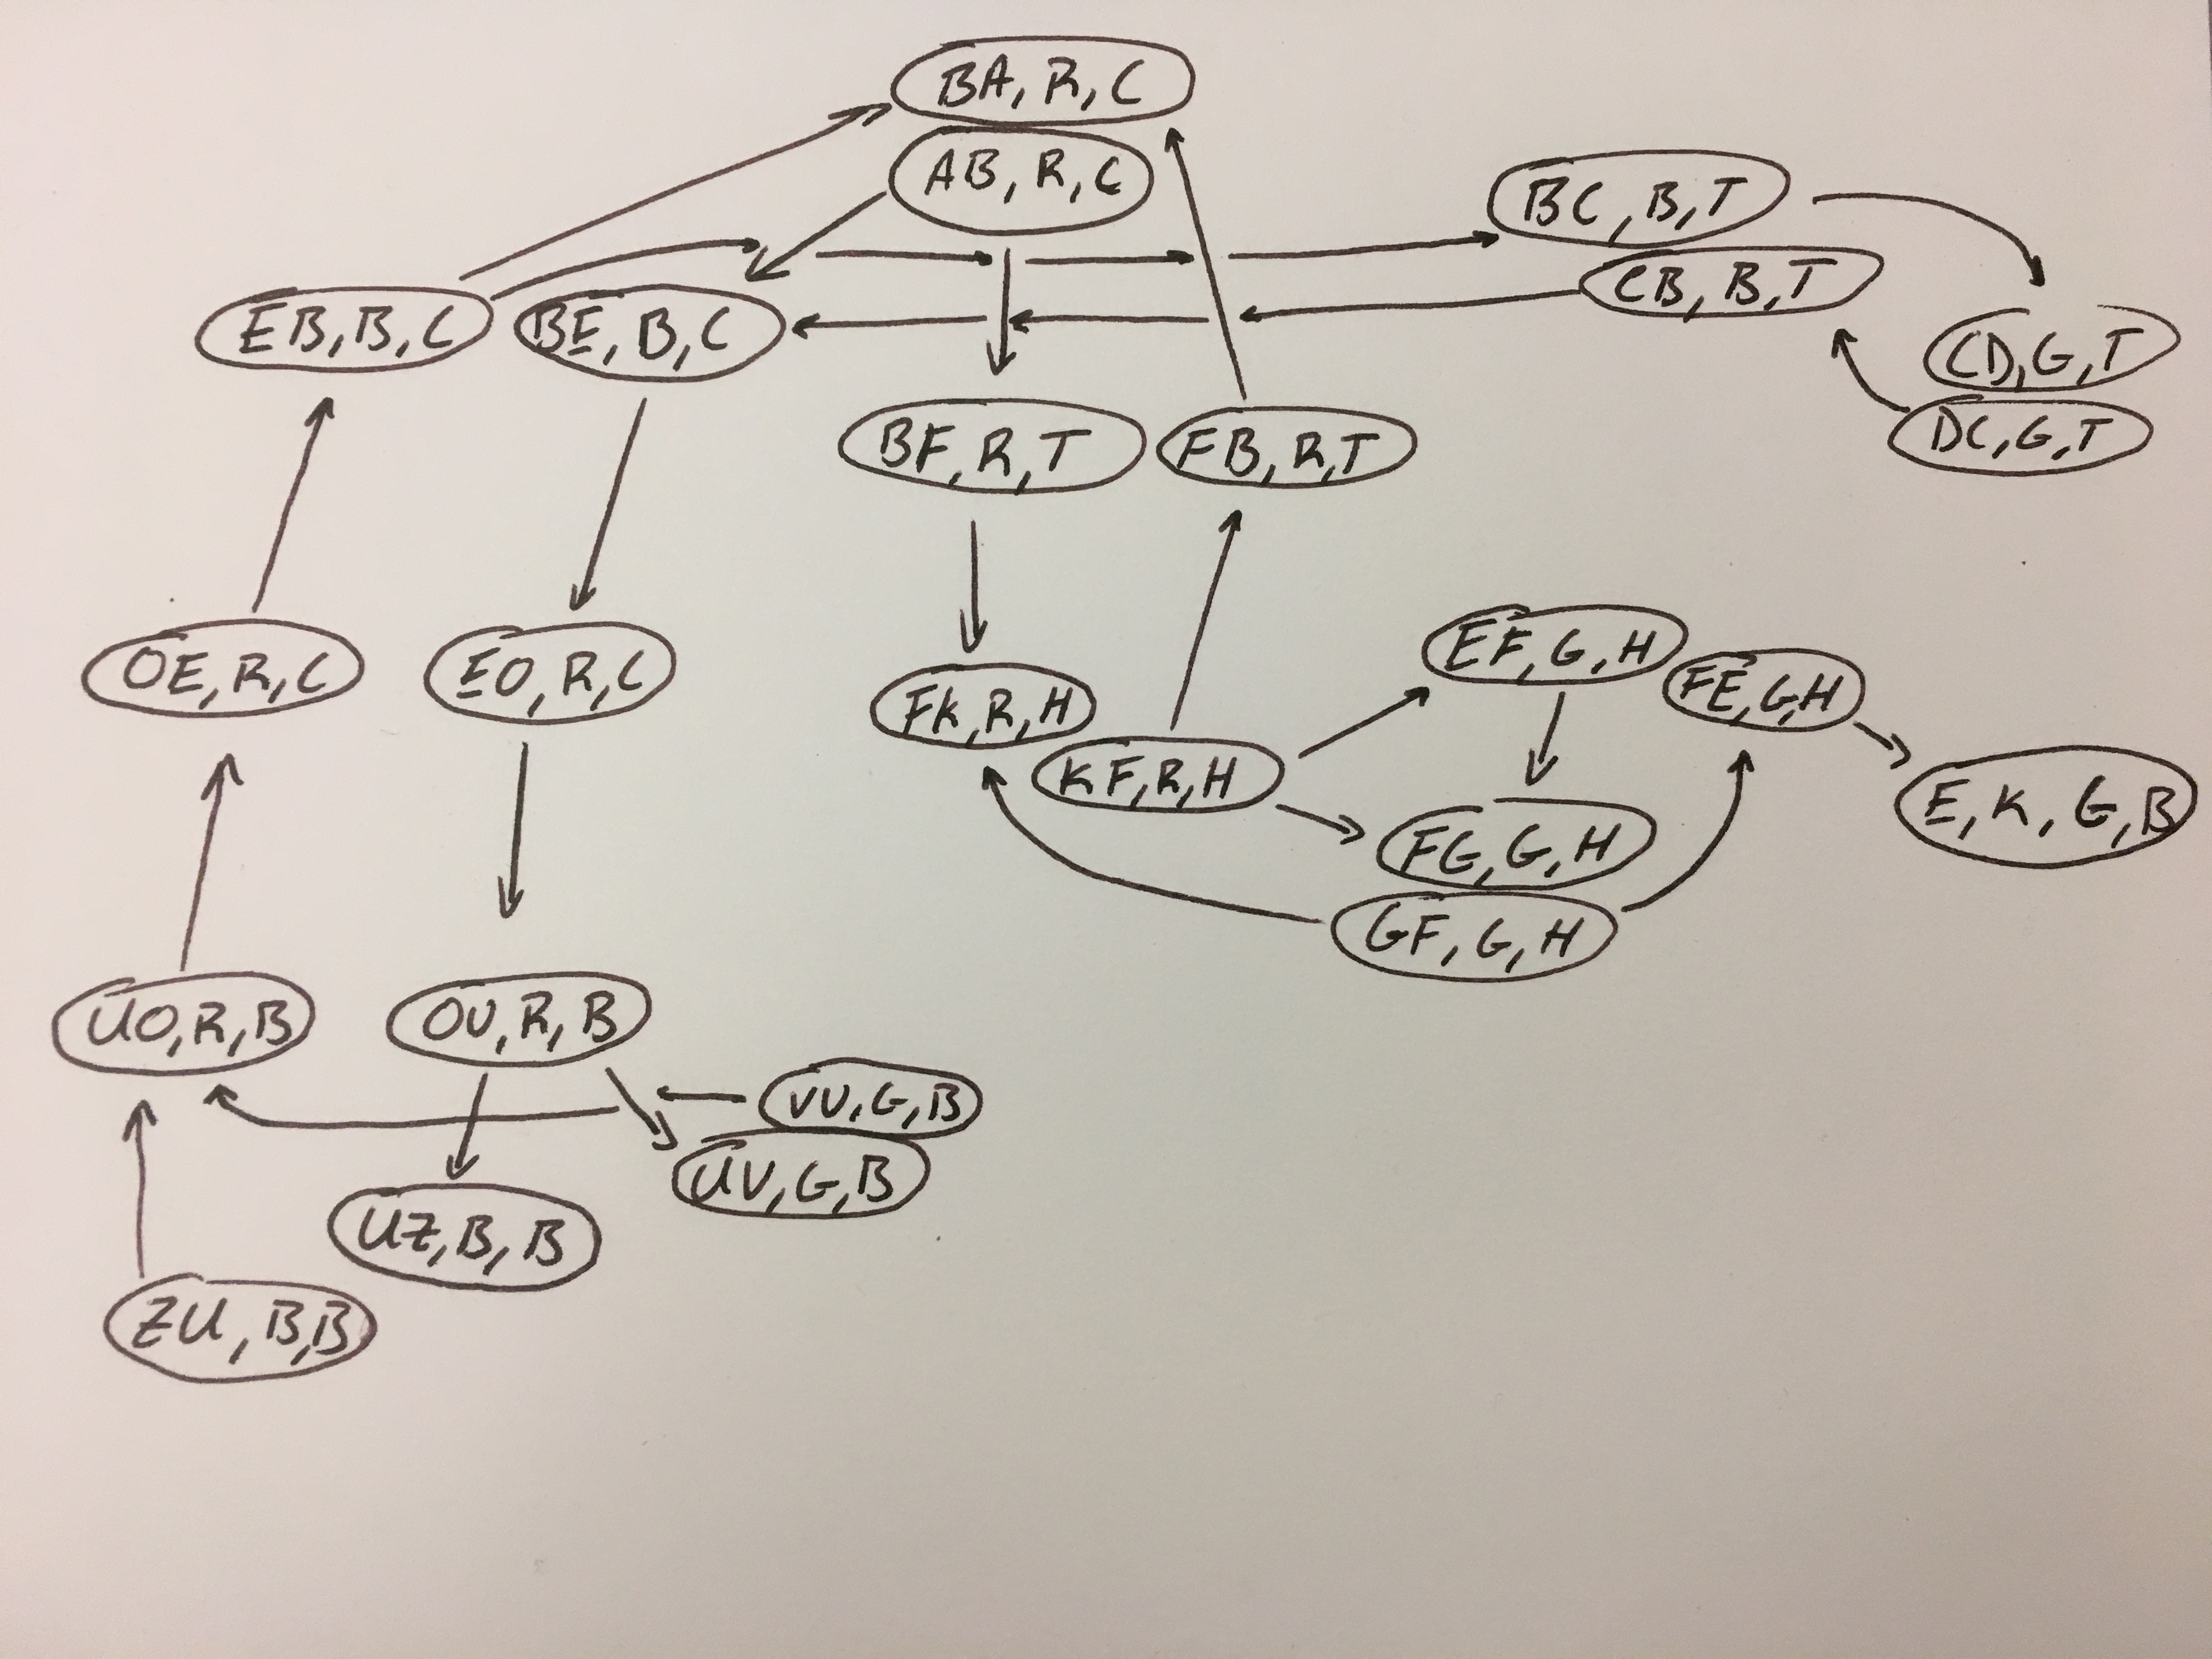
\includegraphics[scale=0.1]{map}
\end{center}
\tab In order to find a solution, a Breadth First Search was necessary. A BFS travels to an edge, and then explores all adjacent edges before continuing onwards to the next layer of adjacent edges. Thus, the BFS algorithm never re-explores an edge in the same direction and continually flows through until it finds an exit. Because of this, it is ensured to find a path to the end given the maze was modeled correctly and that there is in fact a solution. You can think of it as pouring water into the map and having it all trickle down until it reaches the solution, it'll find all the dead ends, but also find a path that gets to the end.
\newpage
\section{The Code}
\linespread{1}
\begin{lstlisting}[caption= Maze Model]
# Container Object, each edge is stored in a hash map as as 
# (start,end):(color, type, [Adjacency List])
Maze = {}

# Read in first line from file,
# that first line is not used in this program so nothing is done with it
text_file = open("input.txt", "r")
text_file.readline()

# For each subsequent line, 
# create one forward traveling and one backwards traveling "node" 
# representing each edge in the Maze
for line in text_file:
    start, end, color, typ = line.split()
    Maze[(start,end)] = (color, typ, [])
    Maze[(end,start)] = (color, typ, [])

# Check start and end nodes and link together adjacent nodes
for key, value in Maze.items():
    for k, v in Maze.items():
       if ((key[1] == k[0]) and (key[0] != k[1]) and (value[0] == v[0] or value[1] == v[1])):
           value[2].append(k)

\end{lstlisting}

Listing 1 displays the code used to generate the Model for my Maze data structure. 

\begin{lstlisting}[caption=BFS]
#Bredth First Search
S = set()
Q = deque([]) # to be used as a queue

root = ('A','B')
goal = ('i','j')

#add root to set and queue
S.add(root)
Q.append(root)

#Backtrace dictionary stored as (child):(parent)
Backtrace = {}
Backtrace[root] = None

while Q:
    current = Q.popleft()
    if current == goal:
        break
    val = Maze[current]
    for n in val[2]:
        if n not in S:
            S.add(n)
            Backtrace[n] = current
            Q.append(n)
\end{lstlisting}

Listing 2 shows the code used to perform a Breadth First Search on my maze data structure, constructing a new Hash Map of nodes to their parent in order to perform a traceback later.

\newpage

\begin{lstlisting}[caption=Traceback]

#Backtrace to build path
path = []
path.append(goal)
node = goal
while current != root:
    current = Backtrace[node]
    path.append(current)
    node = current

\end{lstlisting}

\tab The traceback step constructs the path that was taken to reach the end of the Maze through the use of the BFS algorithm.

\section{Program Output}
The code that I generated results in the following output into the console ... \\\\
The path through the maze takes 49 steps and follows the path : 
[('A', 'B'), ('B', 'E'), ('E', 'O'), ('O', 'U'), ('U', 'V'), ('V', 'a'), ('a', 'f'), ('f', 'Z'), ('Z', 'U'), ('U', 'O'), ('O', 'E'), ('E', 'B'), ('B', 'C'), ('C', 'D'), ('D', 'J'), ('J', 'N'), ('N', 'T'), ('T', 'S'), ('S', 'R'), ('R', 'Q'), ('Q', 'P'), ('P', 'K'), ('K', 'F'), ('F', 'G'), ('G', 'L'), ('L', 'Q'), ('Q', 'W'), ('W', 'b'), ('b', 'a'), ('a', 'Z'), ('Z', 'V'), ('V', 'W'), ('W', 'X'), ('X', 'S'), ('S', 'Y'), ('Y', 'e'), ('e', 'd'), ('d', 'S'), ('S', 'M'), ('M', 'I'), ('I', 'D'), ('D', 'G'), ('G', 'K'), ('K', 'O'), ('O', 'V'), ('V', 'b'), ('b', 'h'), ('h', 'i'), ('i', 'j')] \\~\\

This output suggests that 49 steps were taken and those traversals are displayed in the list. After comparing the number of steps received from the algorithm to the number that I had found when finding a solution by hand, and comparing my path to the path that was generated, I was happy to say that the algorithm I had developed resulted in the exact same solution that I had found by hand.
\end{document}
